\chapter{\textsc {Analyse et calcul d'une loi de commande par retour d'état} }
 \chaptermark{\textsc {Analyse et calcul d'une loi de commande par retour d'état}}
 
	\section{\textsc {Commandabilité du modèle linéarisé}} 
 	
 	\paragraph{}
 		Calcul de la matrice de commandabilité $Co=\begin{bmatrix} B&BA&A^{2}B \end{bmatrix} $:
 		
 		\begin{center}
			
			$Co$=$\begin{bmatrix}
			64.9351&-0.5975&0.0110\\
			0&0.5975&-0.0173\\
			0&0&0.0064
			\end{bmatrix}$	
			 			
		\end{center} 		 
		
		La matrice de commandabilité est triangulaire supérieure ce qui fait que son rang vaut 3 car il n'éxiste aucune relation linéaire entre ses colonnes ou entre ses lignes,\label{Co} \hyperref[Annexe A]{voir Annexe A.}\\
		
		\textbf{Conclusion:} Le modèle linéarisé est bien commandable vu que le rang de la matrice $Co$ est égale au nombre de valeurs propres que possède la matrice $(PI_d-A)$. 
		
		\section{\textsc {La loi de commande par retour d'état}} 
		
		\begin{center}
		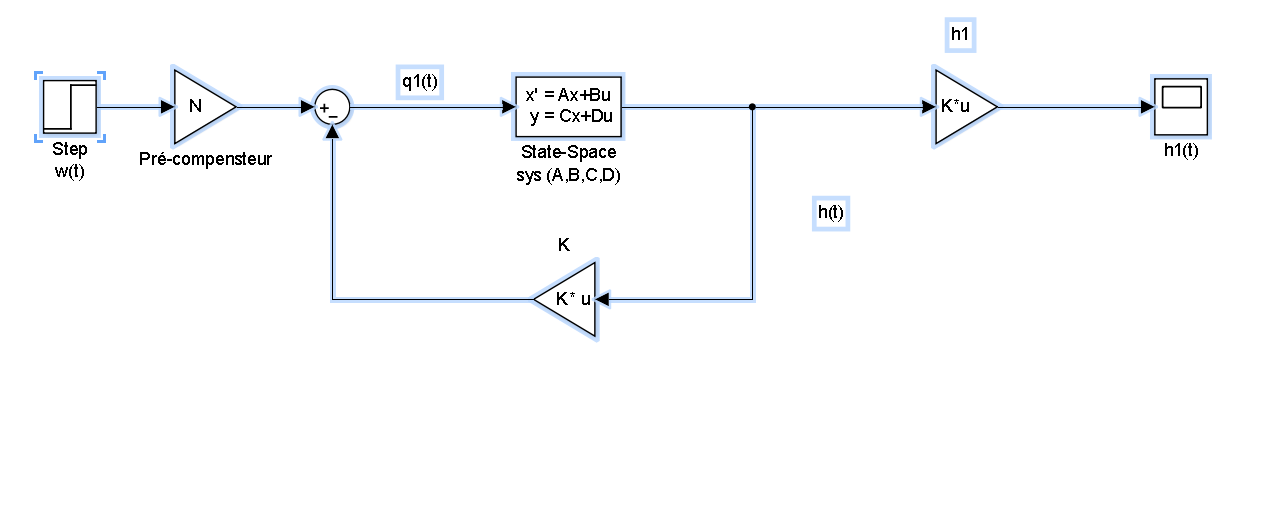
\includegraphics[scale=0.3]{retouretat.PNG} 
		\captionof{figure}{\textit Schéma SIMULINK du système en boucle fermée avec retour d'état}
		\label{fig1}
		\end{center}
		
		\paragraph{} Les matrices du système en boucle fermée deviennent:\\
		
		\begin{center}
			
			$A_{BF}=A-BK$\\
			 $B_{BF}=B$\\
			 $C_{BF}=C$\\
			 $D_{BF}=D=0$			
			
		\end{center}				
		
		\paragraph{}
			Afin de calculer les paramètres du retour d'état soit le gain matriciel $K$ et le pré-compensateur $N$ nous devons choisir des valeurs pour les pôles désirés $P_{des}=\begin{pmatrix} P_1 & P_2 & P_3 \end{pmatrix} $ qui respectent les spécificités du cahier des charges.\\
		
		\paragraph{} Du cours de SLI2 le temps de réponse $t_r =\frac{3}{|Re(vp)|} $, $vp$ : valeur propre. Vu qu'une spécificité dit que $t_r \leqslant 90s$ alors on trouve:\\
		
		\begin{center}
				
				$t_r =\frac{3}{|Re(vp)|}\leqslant 90 $\\[1cm]
				$\Rightarrow|Re(vp)| \geqslant \frac{3}{90} \simeq 0.033 $\\[1cm]
				$\Rightarrow Re(vp) \geqslant 0.033 \wedge Re(vp) \leqslant -0.033$
		\end{center}
		Si $\Rightarrow Re(vp) \geqslant 0.033$ alors notre système est instable, donc la plus lente valeur propre autrement appelée mode dominant doit être inférieur ou égal à $-0.033$.\\\\
		
		Nous choisissons alors les valeurs désirés suivantes: $P_{des}= \begin{bmatrix} P_1&P_2&P_3\end{bmatrix}=\begin{bmatrix} -0.033&-0.15&-0.12 \end{bmatrix} $. Afin de calculer le gain matriciel $K=\begin{bmatrix} K_1 & K_2 & K_3 \end{bmatrix}$ il faut impérativement que le polynôme caractéristique:$ \Psi(A-BK)= \Psi(P_{des})$, autrement dit: $det(PI_d-(A-BK))=(P-P_1)(P-P_2)(P-P_3)$, on trouve:\\
		
		\begin{center}
					
			$\psi(A-BK)$=\\$\Psi(A_{BF})$=$\begin{vmatrix}
			P+0.009202+64.93506K_1&-0.009202-64.93506K_2&64.93506K_3\\
			-0.009202&P+0.019831&-0.010629\\
			 0.000000&-0.010629&P+0.048646
			\end{vmatrix}$\\[1.5cm]
			
			$\Psi(P_{des})=(P+0.033)(P+0.15)(P+0.12)$			
			
		\end{center}
		
		\paragraph{} Par identification on trouve que $K=\begin{bmatrix} 0.0035&0.0170&-0.0141\end{bmatrix}$ la valeur du gain matriciel du retour d'état,\label{K} \hyperref[Annexe B]{voir Annexe B.}\\
		
		\paragraph{} On sait que: $N=\frac{1}{C(-A+BK)^{-1}B+D}$ on obtient au final: $N=0.0108$,\label{N} \hyperref[Annexe C]{Voir Annexe C.}
		
		\begin{center}
		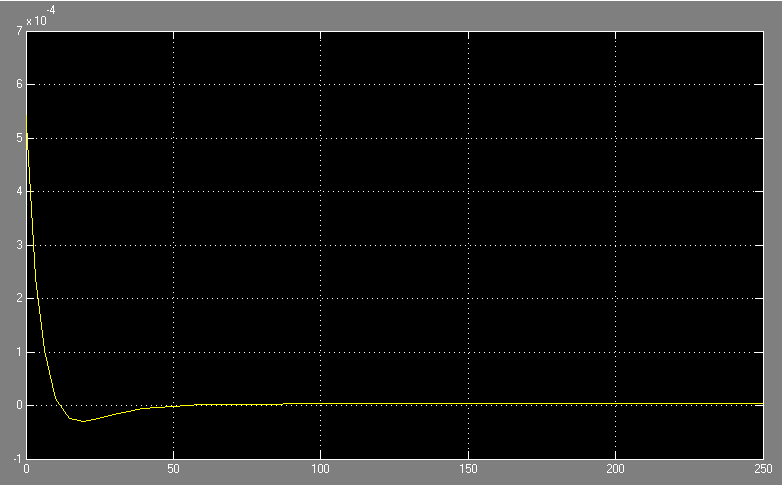
\includegraphics[scale=0.5]{q1(t).PNG} 
		\captionof{figure}{\textit Tracé de $q_1(t)$}
		\label{fig2}
		\end{center}

			\textbf{Remarque:} On remarque de le signal $q_1(t)$ converge vers une valeur nulle, ce qui confirme le bon calcul de la valeur du pré-compensateur qui joue sur le comportement du régime permanent autrement dit sur l'erreur de position. 
		
		\begin{center}
		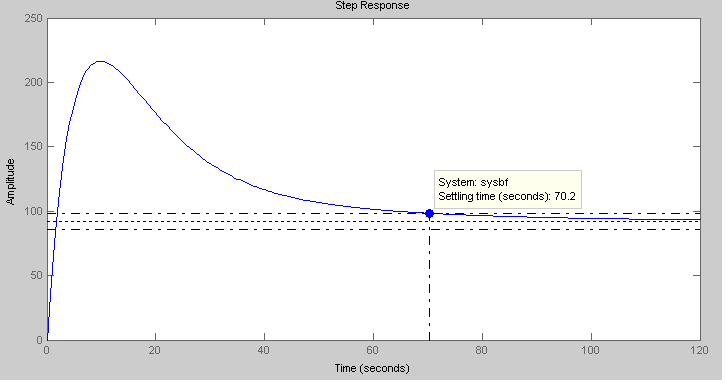
\includegraphics[scale=0.5]{h1(t).PNG} 
		\captionof{figure}{\textit Tracé de $h_1(t)$}
		\label{fig3}
		\end{center}
		
		\textbf{Remarque:} M.GOUAISBAUT nous a imposé d'avoir un temps de réponse $t_{r}  \leqslant 98s$, les valeurs de $P_{des}$ choisies valident la condition mais on observe l'apparition d'un dépassement du à un zéro dominant qu'on ne pourra malheureusement pas enlever, or ça ne pose aucun problème pour le cahier des charges. 
		
		